\documentclass[12pt, a4paper]{article}
\usepackage[utf8]{inputenc}
\usepackage{amsmath}
\usepackage{relsize}
\usepackage{array}
\usepackage{xcolor}
\usepackage{courier}
\usepackage{listings}
\lstset{basicstyle=\footnotesize\ttfamily,breaklines=true}
\lstset{framextopmargin=50pt,frame=bottomline}
\usepackage{tikz}
\usetikzlibrary{calc}
\usepackage{graphicx}
\graphicspath{ {./images/} }
\usepackage{multirow}

\title{CEG3155A Assignment 2}
\author{Jake Wang/*}
\date{\today}

\begin{document}
	\maketitle
	
	\section*{Question I}
	\subsection*{Part a}
	In a number system, there are three digits: 0, 1 and 2. Table 1 defines a ternary half adder. Design a circuit that realizes this half adder using binary coded signals, such that two bits are used for each ternary digit. Let $A = a_1a_0$, $B = b_1b_0$ and $\text{Sum} = s_1s_0$; and note that Report is a binary signal. Use the following coding: $00 = (0)_3$, $01 = (1)_3$ and $10 = (2)_3$. Minimize the cost of the final circuit.
	\begin{center}
		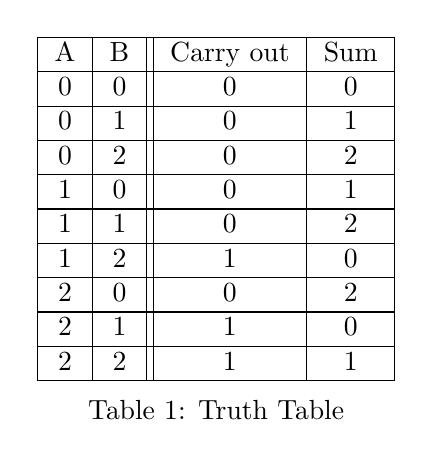
\begin{tikzpicture}
			\node(table)[label=below:Table 1: Truth Table]
			{
				\begin{tabular}{| c | c || c | c |}
					\hline
					A & B & \text{Carry out} & \text{Sum} \\
					\hline
					0 & 0 & 0 & 0 \\
					\hline
					0 & 1 & 0 & 1 \\
					\hline
					0 & 2 & 0 & 2 \\
					\hline
					1 & 0 & 0 & 1 \\
					\hline
					1 & 1 & 0 & 2 \\
					\hline
					1 & 2 & 1 & 0 \\
					\hline
					2 & 0 & 0 & 2 \\
					\hline
					2 & 1 & 1 & 0 \\
					\hline
					2 & 2 & 1 & 1 \\
					\hline
				\end{tabular}
			};
		\end{tikzpicture}
	\end{center}
	
	Convert the truth table to binary representation:
	\begin{center}
		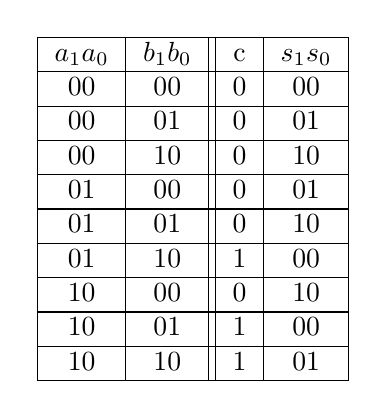
\begin{tikzpicture}
			\node(table)
			{
				\begin{tabular}{| c | c || c | c |}
					\hline
					$a_1a_0$ & $b_1b_0$ & c & $s_1s_0$ \\
					\hline
					00 & 00 & 0 & 00 \\
					\hline
					00 & 01 & 0 & 01 \\
					\hline
					00 & 10 & 0 & 10 \\
					\hline
					01 & 00 & 0 & 01 \\
					\hline
					01 & 01 & 0 & 10 \\
					\hline
					01 & 10 & 1 & 00 \\
					\hline
					10 & 00 & 0 & 10 \\
					\hline
					10 & 01 & 1 & 00 \\
					\hline
					10 & 10 & 1 & 01 \\
					\hline
				\end{tabular}
			};
		\end{tikzpicture}
	\end{center}
	
	K-map for $c$:
	\begin{center}
		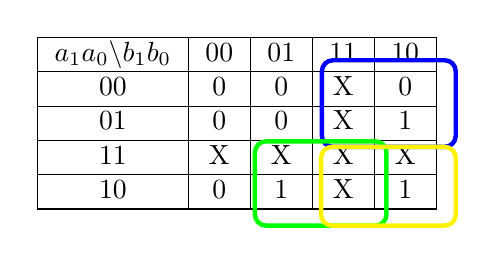
\begin{tikzpicture}
			\node(table)
			{
				\begin{tabular}{| c | c | c | c | c |}
					\hline
					$a_1a_0$\textbackslash$b_1b_0$ & 00 & 01 & 11 & 10 \\
					\hline
					00 & 0 & 0 & X & 0 \\
					\hline
					01 & 0 & 0 & X & 1 \\
					\hline
					11 & X & X & X & X \\
					\hline
					10 & 0 & 1 & X & 1 \\
					\hline
				\end{tabular}
			};
			\draw [blue, ultra thick, rounded corners] (1.08, -0.3) rectangle (2.78, 0.8);
			\draw [green, ultra thick, rounded corners] (0.23, -1.3) rectangle (1.9, -0.23);
			\draw [yellow, ultra thick, rounded corners] (1.07, -1.3) rectangle (2.78, -0.3);
		\end{tikzpicture}
	\end{center}
	$$c = a_1b_0 + a_1b_1 + a_0b_1$$
	
	K-map for $s_1$:
	\begin{center}
		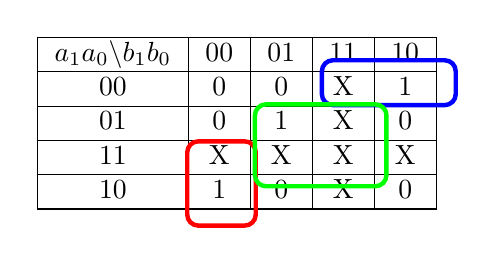
\begin{tikzpicture}
			\node(table)
			{
				\begin{tabular}{| c | c | c | c | c |}
					\hline
					$a_1a_0$\textbackslash$b_1b_0$ & 00 & 01 & 11 & 10 \\
					\hline
					00 & 0 & 0 & X & 1 \\
					\hline
					01 & 0 & 1 & X & 0 \\
					\hline
					11 & X & X & X & X \\
					\hline
					10 & 1 & 0 & X & 0 \\
					\hline
				\end{tabular}
			};
			\draw [red, ultra thick, rounded corners] (-0.63, -1.3) rectangle (0.24, -0.23);
			\draw [blue, ultra thick, rounded corners] (1.08, 0.23) rectangle (2.78, 0.8);
			\draw [green, ultra thick, rounded corners] (0.23, -0.8) rectangle (1.9, 0.24);
		\end{tikzpicture}
	\end{center}
	$$s_1 = a_1b_1'b_0' + a_0b_0 + a_1'a_0'b_1$$
	
	K-map for $s_0$:
	\begin{center}
		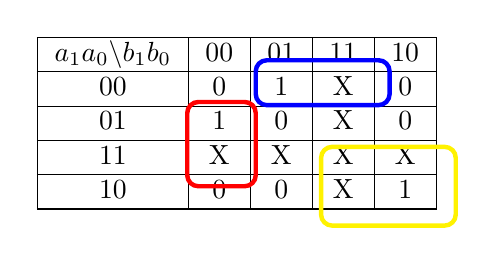
\begin{tikzpicture}
			\node(table)
			{
				\begin{tabular}{| c | c | c | c | c |}
					\hline
					$a_1a_0$\textbackslash$b_1b_0$ & 00 & 01 & 11 & 10 \\
					\hline
					00 & 0 & 1 & X & 0 \\
					\hline
					01 & 1 & 0 & X & 0 \\
					\hline
					11 & X & X & X & X \\
					\hline
					10 & 0 & 0 & X & 1 \\
					\hline
				\end{tabular}
			};
			\draw [red, ultra thick, rounded corners] (-0.63, -0.8) rectangle (0.24, 0.27);
			\draw [blue, ultra thick, rounded corners] (0.24, 0.23) rectangle (1.94, 0.8);
			\draw [yellow, ultra thick, rounded corners] (1.07, -1.3) rectangle (2.78, -0.3);
		\end{tikzpicture}
	\end{center}
	$$s_0 = a_0b_1'b_0' + a_1'a_0'b_0 + a_1b_1$$
	
	\subsection*{Part b}
	Design the circuit of the ternary full-adder using the method described in part a.
	\\
	
	Circuit Design:
	\begin{center}
		\begin{tikzpicture}
			\node(picture) {\includegraphics{Q1Design.pdf}};
		\end{tikzpicture}
	\end{center}
	
	
	\section*{Question II}
	\subsection*{Part a}
	What is the critical path in the multiplier in figure 1? What is the delay of this path in terms of the number of logic gates?
	\begin{center}
		\begin{tikzpicture}
			\node(picture)[label=below:Figure 1: Row Multiplier] {\includegraphics{Q2RowMultiplier.png}};
		\end{tikzpicture}
	\end{center}
	
	The critical path is shown as below:
	\begin{center}
		\begin{tikzpicture}
			\node(picture) {\includegraphics[scale=0.5]{Q2CriticalPath.png}};
		\end{tikzpicture}
	\end{center}
	
	The delay of the path:
	
	In the path, there are 6 carry outputs and 2 sum outputs. For each carry output, the signal passes through one XOR gate, one AND gate and one OR gate; for each sum output, the signal passes through 2 XOR gates. So the total delay is:
	$$6 \times (1 + 1 + 1) + 2 \times 2 = 24\ (\text{gates})$$
	
	\subsection*{Part b}
	Show that the multiplication of two n-digit numbers in base $B$ gives a product with no more than $2n$ digits.
	
	The maximum value of an n-digit number in base $B$ is
		$$B ^ n - 1$$
	
	Then, the maximum value of the product of two n-digit numbers is
		$$(B ^ n - 1) ^ 2 = B ^ {2n} - 2B^n + 1$$ 

	Since $B > 1$ and $n \ge 1$,
		$$-2B ^ n + 1 < 0$$
		$$(B ^ n - 1) ^ 2 < B ^ {2n}$$
		$$(B ^ n - 1) ^ 2 \le B ^ {2n} - 1$$
	
	i.e. The product is less or equal $B ^ {2n} - 1$.
	\\
	
	Therefore, the number of digits of the product will not exceed $2n$.

	\section*{Question III}
	\subsection*{Part a}
	A sequential circuit contains two inputs, $w_1$ and $w_2$, and one output, $z$. Its function is to compare the data sequences of the two inputs. If $w_1 = w_2$ for any four consecutive clock periods, the circuit produces $z = 1$; otherwise $z = 0$. For example:
	
	$$w_1 = 0110111000110$$
	$$w_2 = 1110101000111$$
	$$z = 0000100001110$$
	\\
	Derive the appropriate circuit.
	\\
	
	State Table:
	\begin{center}
		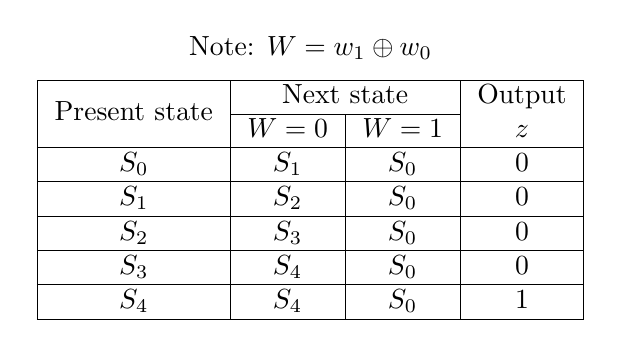
\begin{tikzpicture}
			\node(table)[label=above:{Note: $W = w_1 \oplus w_0$}]
			{
				\begin{tabular}{| c | c | c | c |}
					\hline
					\multirow{2}{*}{Present state} & \multicolumn{2}{c |}{Next state} & Output \\
					\cline{2-3} & $W = 0$ & $W = 1$ & $z$ \\
					\hline
					$S_0$ & $S_1$ & $S_0$ & 0 \\
					\hline
					$S_1$ & $S_2$ & $S_0$ & 0 \\
					\hline
					$S_2$ & $S_3$ & $S_0$ & 0 \\
					\hline
					$S_3$ & $S_4$ & $S_0$ & 0 \\
					\hline
					$S_4$ & $S_4$ & $S_0$ & 1 \\
					\hline
				\end{tabular}
			};
		\end{tikzpicture}
	\end{center}
	
	
	Transition Table (DFF):
	\begin{center}
		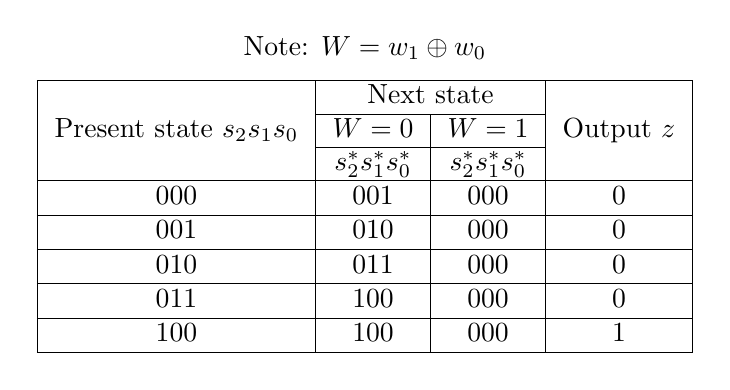
\begin{tikzpicture}
			\node(table)[label=above:{Note: $W = w_1 \oplus w_0$}]
			{
				\begin{tabular}{| c | c | c | c |}
					\hline
					\multirow{3}{*}{Present state $s_2s_1s_0$} & \multicolumn{2}{c |}{Next state} & \multirow{3}{*}{Output $z$} \\
					\cline{2-3} & $W = 0$ & $W = 1$ &  \\
					\cline{2-3} & $s_2^*s_1^*s_0^*$ & $s_2^*s_1^*s_0^*$ &  \\
					\hline
					$000$ & $001$ & $000$ & 0 \\
					\hline
					$001$ & $010$ & $000$ & 0 \\
					\hline
					$010$ & $011$ & $000$ & 0 \\
					\hline
					$011$ & $100$ & $000$ & 0 \\
					\hline
					$100$ & $100$ & $000$ & 1 \\
					\hline
				\end{tabular}
			};
		\end{tikzpicture}
	\end{center}
	
	K-map Optimization:
	
	K-map for $s_2^*$:
	\begin{center}
		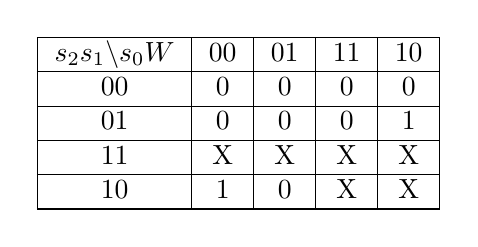
\begin{tikzpicture}
			\node(table)
			{
				\begin{tabular}{| c | c | c | c | c |}
					\hline
					$s_2s_1$\textbackslash$s_0W$ & 00 & 01 & 11 & 10 \\
					\hline
					00 & 0 & 0 & 0 & 0 \\
					\hline
					01 & 0 & 0 & 0 & 1 \\
					\hline
					11 & X & X & X & X \\
					\hline
					10 & 1 & 0 & X & X \\
					\hline
				\end{tabular}
			};
		\end{tikzpicture}
	\end{center}
	$$s_2^* = s_2W' + s_1s_0W'$$
	
	K-map for $s_1^*$:
	\begin{center}
		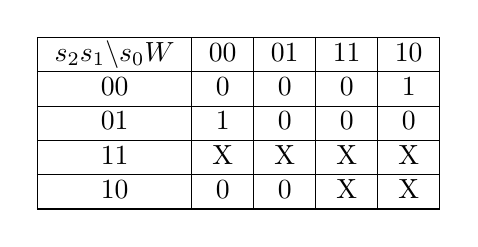
\begin{tikzpicture}
			\node(table)
			{
				\begin{tabular}{| c | c | c | c | c |}
					\hline
					$s_2s_1$\textbackslash$s_0W$ & 00 & 01 & 11 & 10 \\
					\hline
					00 & 0 & 0 & 0 & 1 \\
					\hline
					01 & 1 & 0 & 0 & 0 \\
					\hline
					11 & X & X & X & X \\
					\hline
					10 & 0 & 0 & X & X \\
					\hline
				\end{tabular}
			};
		\end{tikzpicture}
	\end{center}
	$$s_1^* = s_1's_0W' + s_1s_0'W'$$

	K-map for $s_0^*$:
	\begin{center}
		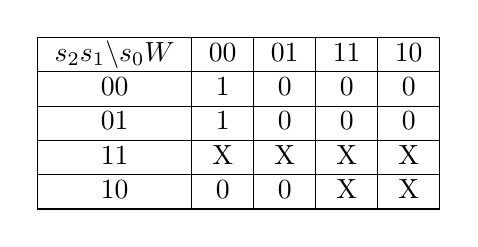
\begin{tikzpicture}
			\node(table)
			{
				\begin{tabular}{| c | c | c | c | c |}
					\hline
					$s_2s_1$\textbackslash$s_0W$ & 00 & 01 & 11 & 10 \\
					\hline
					00 & 1 & 0 & 0 & 0 \\
					\hline
					01 & 1 & 0 & 0 & 0 \\
					\hline
					11 & X & X & X & X \\
					\hline
					10 & 0 & 0 & X & X \\
					\hline
				\end{tabular}
			};
		\end{tikzpicture}
	\end{center}
	$$s_0^* = s_2's_0'W'$$
	
	K-map for $z$:
	\begin{center}
		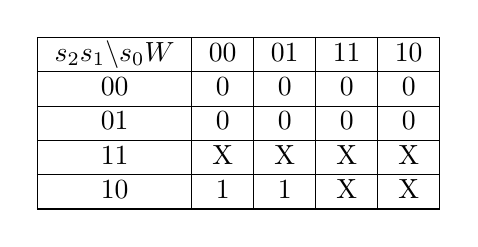
\begin{tikzpicture}
			\node(table)
			{
				\begin{tabular}{| c | c | c | c | c |}
					\hline
					$s_2s_1$\textbackslash$s_0W$ & 00 & 01 & 11 & 10 \\
					\hline
					00 & 0 & 0 & 0 & 0 \\
					\hline
					01 & 0 & 0 & 0 & 0 \\
					\hline
					11 & X & X & X & X \\
					\hline
					10 & 1 & 1 & X & X \\
					\hline
				\end{tabular}
			};
		\end{tikzpicture}
	\end{center}
	$$z = s_2$$
	
	Circuit Design:
	\begin{center}
		\begin{tikzpicture}
			\node(picture) {\includegraphics[scale=0.8]{Q3PaDesign.pdf}};
		\end{tikzpicture}
	\end{center}
	

	\subsection*{Part b}
	Write the finite state machine (FSM) VHDL code described in part a.
	
	\begin{lstlisting}[language=vhdl]
library ieee;
use ieee.std_logic_1164.all;

entity SequenceComparator is
    port (
        w1, w0: in std_logic;
        CLK, RESETN: in std_logic;
        z: out std_logic
    );
end;

architecture Structural of SequenceComparator is
    component enARdFF_2 IS
        port (
            i_resetBar: in std_logic;
            i_d: in std_logic;
            i_enable: in std_logic;
            i_clock: in std_logic;
            o_q, o_qBar: OUT std_logic
        );
    end component;
    
    signal signalNotW: std_logic;
    signal signalS: std_logic_vector(2 downto 0);
begin
    signalNotW <= w1 xnor w0;
    
    s2DFF: enARdFF_2
        port map (
            i_resetBar => RESETN,
            i_d => (signalS(2) and signalNotW) or (signalS(1) and signalS(0) and signalNotW),
            i_enable => '1',
            i_clock => CLK,
            o_q => signalS(2)
        );
    
    s1DFF: enARdFF_2
        port map (
            i_resetBar => RESETN,
            i_d => ((not signalS(1)) and signalS(0) and signalNotW) or (signalS(1) and (not signalS(0)) and signalNotW),
            i_enable => '1',
            i_clock => CLK,
            o_q => signalS(1)
        );
    
    s0DFF: enARdFF_2
        port map (
            i_resetBar => RESETN,
            i_d => (not signalS(2)) and (not signalS(0)) and signalNotW,
            i_enable => '1',
            i_clock => CLK,
            o_q => signalS(0)
        );
    z <= signalS(2);
end;
	\end{lstlisting}
	
	\subsection*{Part c}
	Design a modulo-6 counter, which counts in the following sequence: 0, 1, 2, 3, 4, 5, 0, 1, 2 ... The counter counts the clock edges if its signal permit, $w$, is equal to 1. Use D-type flip-flops in your circuit.
	
	State Table:
	\begin{center}
		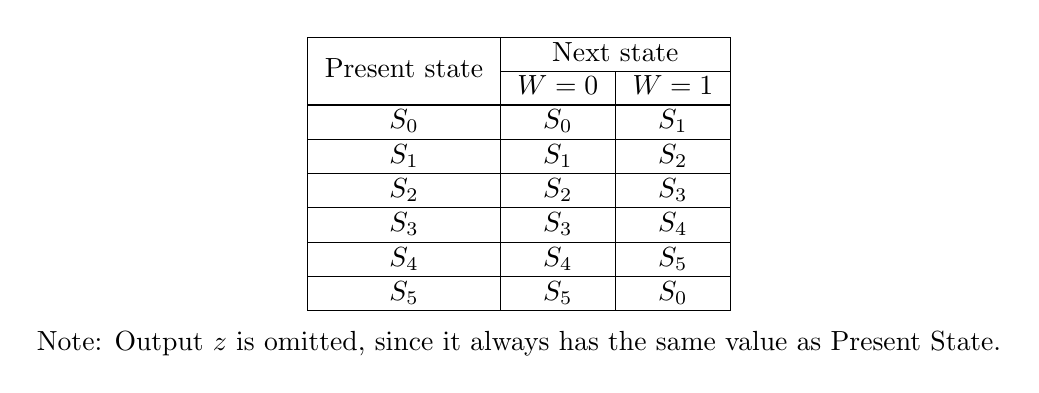
\begin{tikzpicture}
			\node(table)[label=below:{Note: Output $z$ is omitted, since it always has the same value as Present State.}]
			{
				\begin{tabular}{| c | c | c |}
					\hline
					\multirow{2}{*}{Present state} & \multicolumn{2}{c |}{Next state}\\
					\cline{2-3} & $W = 0$ & $W = 1$ \\
					\hline
					$S_0$ & $S_0$ & $S_1$ \\
					\hline
					$S_1$ & $S_1$ & $S_2$ \\
					\hline
					$S_2$ & $S_2$ & $S_3$ \\
					\hline
					$S_3$ & $S_3$ & $S_4$ \\
					\hline
					$S_4$ & $S_4$ & $S_5$ \\
					\hline
					$S_5$ & $S_5$ & $S_0$ \\
					\hline
				\end{tabular}
			};
		\end{tikzpicture}
	\end{center}
	
	
	Transition Table (DFF):
	\begin{center}
		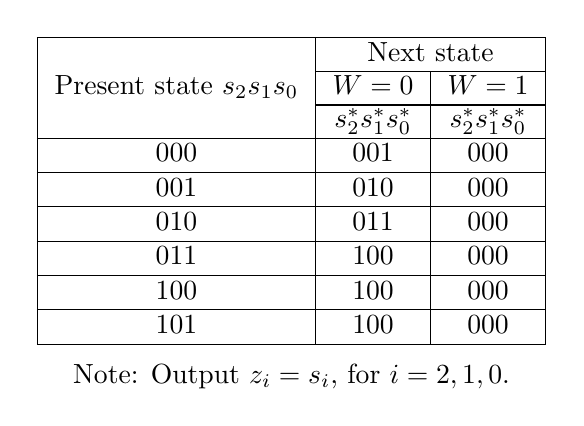
\begin{tikzpicture}
			\node(table)[label=below:{Note: Output $z_i = s_i$, for $i = 2, 1, 0$.}]
			{
				\begin{tabular}{| c | c | c | c |}
					\hline
					\multirow{3}{*}{Present state $s_2s_1s_0$} & \multicolumn{2}{c |}{Next state} \\
					\cline{2-3} & $W = 0$ & $W = 1$ \\
					\cline{2-3} & $s_2^*s_1^*s_0^*$ & $s_2^*s_1^*s_0^*$ \\
					\hline
					$000$ & $001$ & $000$ \\
					\hline
					$001$ & $010$ & $000$ \\
					\hline
					$010$ & $011$ & $000$ \\
					\hline
					$011$ & $100$ & $000$ \\
					\hline
					$100$ & $100$ & $000$ \\
					\hline
					$101$ & $100$ & $000$ \\
					\hline
				\end{tabular}
			};
		\end{tikzpicture}
	\end{center}
	
	K-map Optimization:
	
	K-map for $s_2^*$:
	\begin{center}
		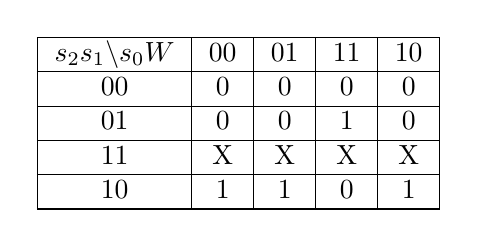
\begin{tikzpicture}
			\node(table)
			{
				\begin{tabular}{| c | c | c | c | c |}
					\hline
					$s_2s_1$\textbackslash$s_0W$ & 00 & 01 & 11 & 10 \\
					\hline
					00 & 0 & 0 & 0 & 0 \\
					\hline
					01 & 0 & 0 & 1 & 0 \\
					\hline
					11 & X & X & X & X \\
					\hline
					10 & 1 & 1 & 0 & 1 \\
					\hline
				\end{tabular}
			};
		\end{tikzpicture}
	\end{center}
	$$s_2^* = s_2s_0' + s_2W' + s_1s_0W$$
	
	K-map for $s_1^*$:
	\begin{center}
		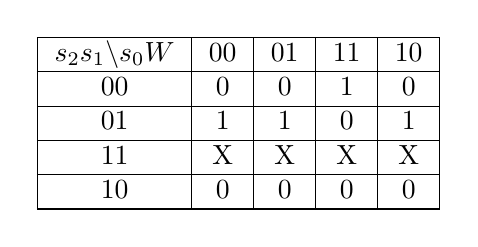
\begin{tikzpicture}
			\node(table)
			{
				\begin{tabular}{| c | c | c | c | c |}
					\hline
					$s_2s_1$\textbackslash$s_0W$ & 00 & 01 & 11 & 10 \\
					\hline
					00 & 0 & 0 & 1 & 0 \\
					\hline
					01 & 1 & 1 & 0 & 1 \\
					\hline
					11 & X & X & X & X \\
					\hline
					10 & 0 & 0 & 0 & 0 \\
					\hline
				\end{tabular}
			};
		\end{tikzpicture}
	\end{center}
	$$s_1^* = s_1s_0' + s_1W' + s_2's_1's_0W$$
	
	K-map for $s_0^*$:
	\begin{center}
		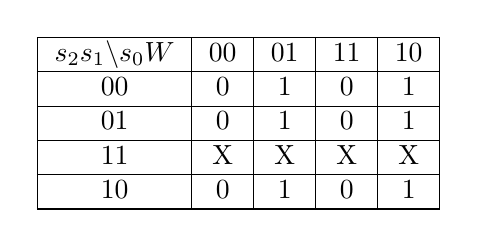
\begin{tikzpicture}
			\node(table)
			{
				\begin{tabular}{| c | c | c | c | c |}
					\hline
					$s_2s_1$\textbackslash$s_0W$ & 00 & 01 & 11 & 10 \\
					\hline
					00 & 0 & 1 & 0 & 1 \\
					\hline
					01 & 0 & 1 & 0 & 1 \\
					\hline
					11 & X & X & X & X \\
					\hline
					10 & 0 & 1 & 0 & 1 \\
					\hline
				\end{tabular}
			};
		\end{tikzpicture}
	\end{center}
	$$s_0^* = s_0'W + s_0W' = s_0 \oplus W$$
	
	Circuit Design:
	\begin{center}
		\begin{tikzpicture}
			\node(picture){\includegraphics{Q3PcDesign.pdf}};
		\end{tikzpicture}
	\end{center}

	\section*{Question IV}
	Draw the synchronization diagrams of the figures 2 and 3, and show the difference between inputs and outputs of a Moore FSM and another of a Mealy FSM.
	
	\begin{center}
		\begin{tikzpicture}
			\node(picture)[label=below:Figure 2: Mealy FSM] {\includegraphics{Q4Mealy.png}};
		\end{tikzpicture}
	\end{center}
	
	\begin{center}
		\begin{tikzpicture}
			\node(picture)[label=below:Figure 3: Moore FSM] {\includegraphics{Q4Moore.png}};
		\end{tikzpicture}
	\end{center}
	
	\begin{center}
		\begin{tikzpicture}
			\node(picture) {\includegraphics[scale=0.75]{Q4Waveform.pdf}};
		\end{tikzpicture}
	\end{center}
	
	\section*{Bonus Question}
	Demonstrate, using a synchronization diagram, the correct operation of a D-type flip-flop as shown in figure 4 and presented in class.
	\begin{center}
		\begin{tikzpicture}
			\node(picture)[label=below:Figure 4: D Flip-flop in master slave configuration] {\includegraphics{QBonus.png}};
		\end{tikzpicture}
	\end{center}
	
	\begin{center}
		\begin{tikzpicture}
			\node(picture)[label=below:The D flip-flop is only triggered at a rising clock edge.]
			{
				\includegraphics{QBonusWaveform.pdf}
			};
		\end{tikzpicture}
	\end{center}
	
\end{document}
